\title{Machine Learning Practical - Assignment 2}
\author{s1247438}
\documentclass[12pt]{article}
\usepackage{caption}
\usepackage{subcaption}
\usepackage[pdftex]{graphicx} 
\usepackage[margin=1in]{geometry}    
\usepackage{float}

\begin{document}

\maketitle


\subsection*{Introduction}
This coursework is focused on training a multi-layered neural network for digit classification on the MINST dataset. The aim of this coursework is to explore effects of these topics : activation layer choice, data augmentation and batch normalization.


\subsection*{Methodology}

The neural network built for the purposes of this assignment is based on the Lab session code provided. Unless otherwise specified the parameters used for the experiments in this paper are included in table \ref{tab:model}. The new additions required for the exploring the mentioned topics include ArcTan and Batch layers as well as multiple functions for data augmentation. Various parameters for each technique were tested where possible.


\begin{table}[H]
\centering
\begin{tabular}[h]{| c | c |}
\hline
model & 3 Affine 2 Relu   \\
\hline
error & cross-entropy softmax   \\
\hline
learning rule & momentum   \\
\hline
learning rate & 0.01\\
\hline 
batch size & 100   \\
\hline
momentum & 0.9   \\
\hline
\end{tabular} 
\caption{Model parameters}
\label{tab:model}
\end{table}




\section*{Task 1 - Layer Choice}

The first section explores how the choice of non-linear activation functions affects the model performance. The activation functions include Sigmoid, Relu, TanH, ArcTan and Elu as displayed on figure \ref{fig:models}.  

\begin{figure}[H]
\centering
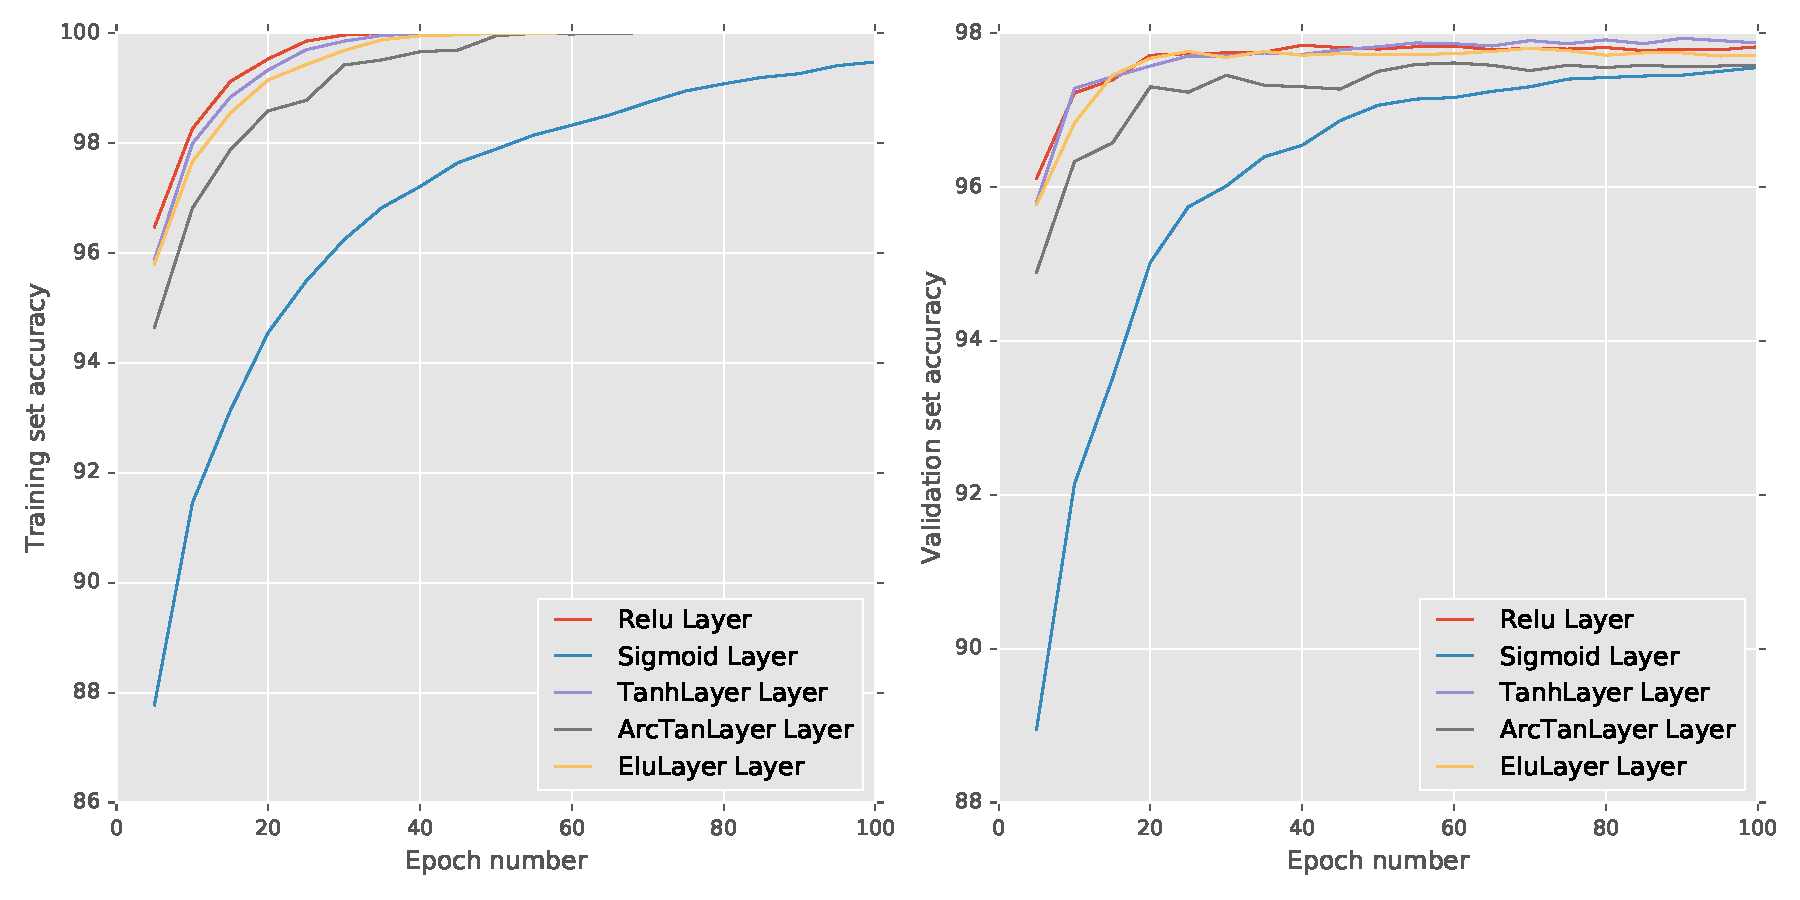
\includegraphics[width=\textwidth]{models_compare.pdf}

  \caption{Effect of the activation layer choice on performance.}
  \label{fig:models}
\end{figure}

The lowest performing function was sigmoid, as it has some key problems. The main is saturation, this occurs when the function outputs values close to 0 or 1, resulting in the gradient being almost 0. Preventing signals going further back into the network. These values can occur naturally from the data but a likely cause is also inappropriate weight initialization. 

The ArcTan and Tanh functions are both prone to saturation as well, but have an advantage of being centred around 0. The difference between performance of ArcTan and TanH should be caused by the difference in the shape of their differentials.

Elu and ReLu functions do not have the problem with saturation and should therefore perform better. The ELU parameter wasn't explored in depth as it should have been made learn-able rather than constant. However Relu achieved the highest performance, demonstrating why it is a good common choice.

\section*{Task 2 - Data Augmentation}

This section explores the effect of different types of data augmentation on the performance of a neural network trained on the MNIST dataset. Data augmentation creates new data points by applying small transformations to the existing dataset aiming to create a more robust final model. The explored augmentations below are : shift, color variation, zoom and a combination of these. 

Shift data augmentation works in a following way. A part (25\%) of randomly chosen data in each batch during training is shifted, moved in a random combination of directions up, down, left, right. Even though the digits are centred minor shifts should improve performance as they give a better representation of the data. Different sizes of shifts were explored in figure \ref{fig:shift}. The experiments show an improvement in performance when applying a very minor shift to the data, as they give a better representation of shape for each digit.



\begin{figure}[H]
\centering
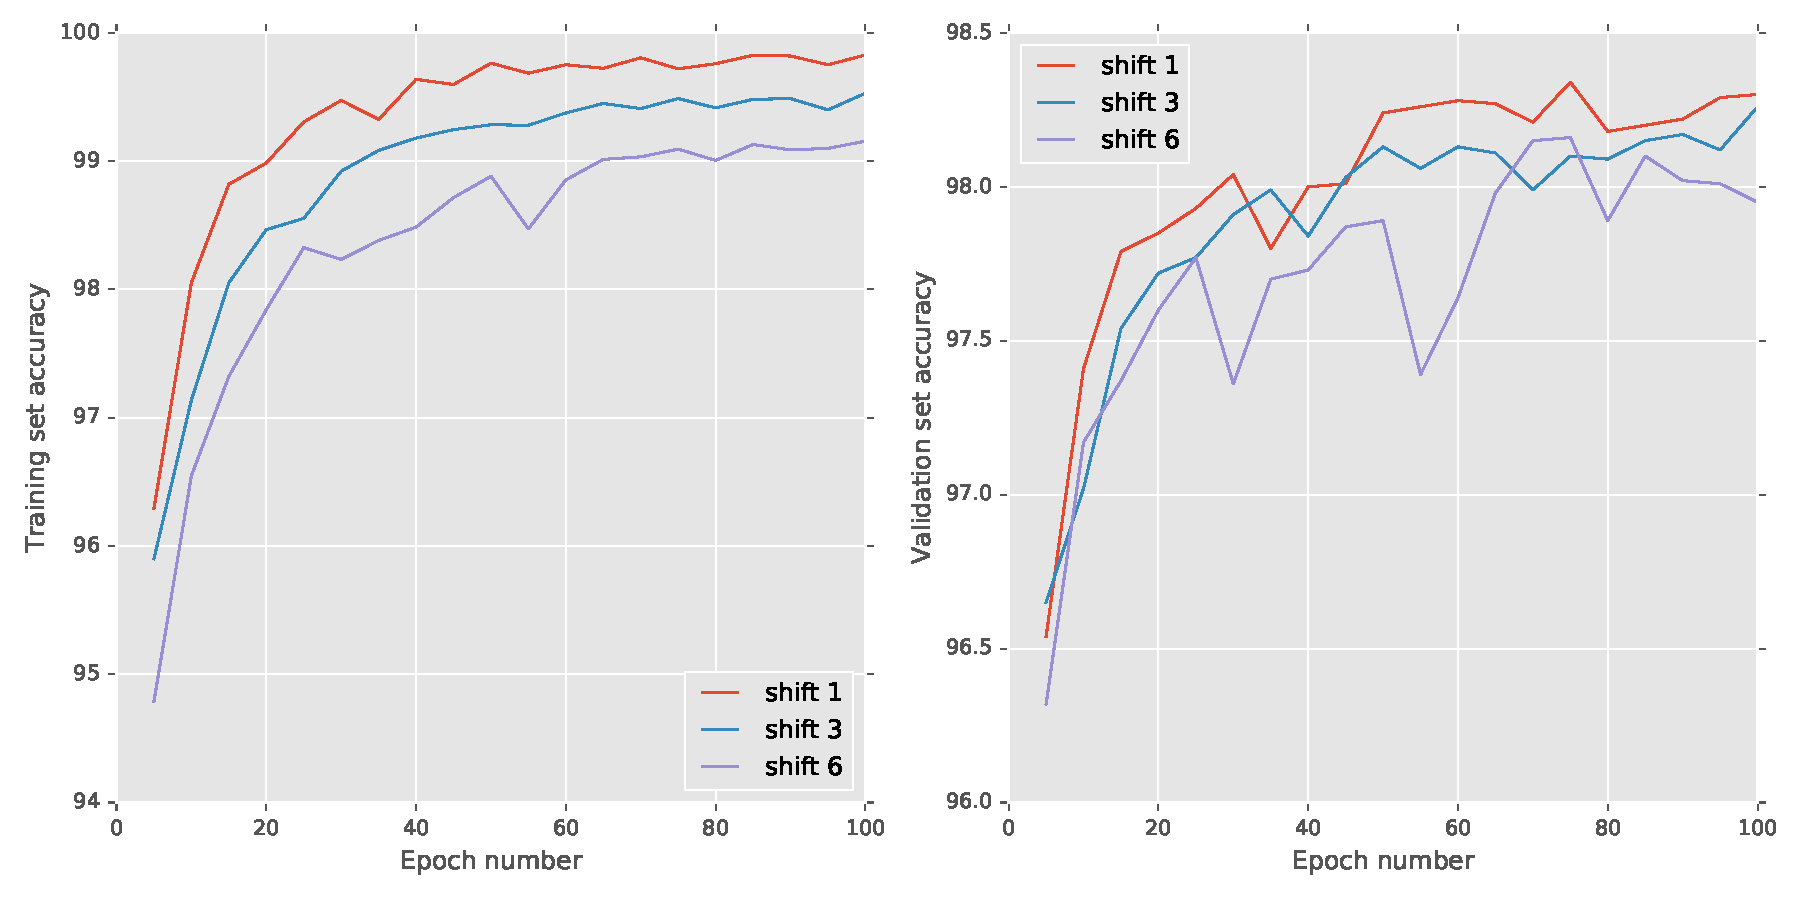
\includegraphics[width=\textwidth]{shift_compare.pdf}

  \caption{Effect of applying shift augmentation to training data.}
  \label{fig:shift}
\end{figure}

A common technique in data augmentation is introducing random noise or color variations. Random noise should not work in this case as the dataset is cleaned. The color variation, making some digits darker or lighter was explored with different strengths on figure \ref{fig:noise} which displays minimal improvement as the color seems to be normalised to an extent.

\begin{figure}[H]
\centering
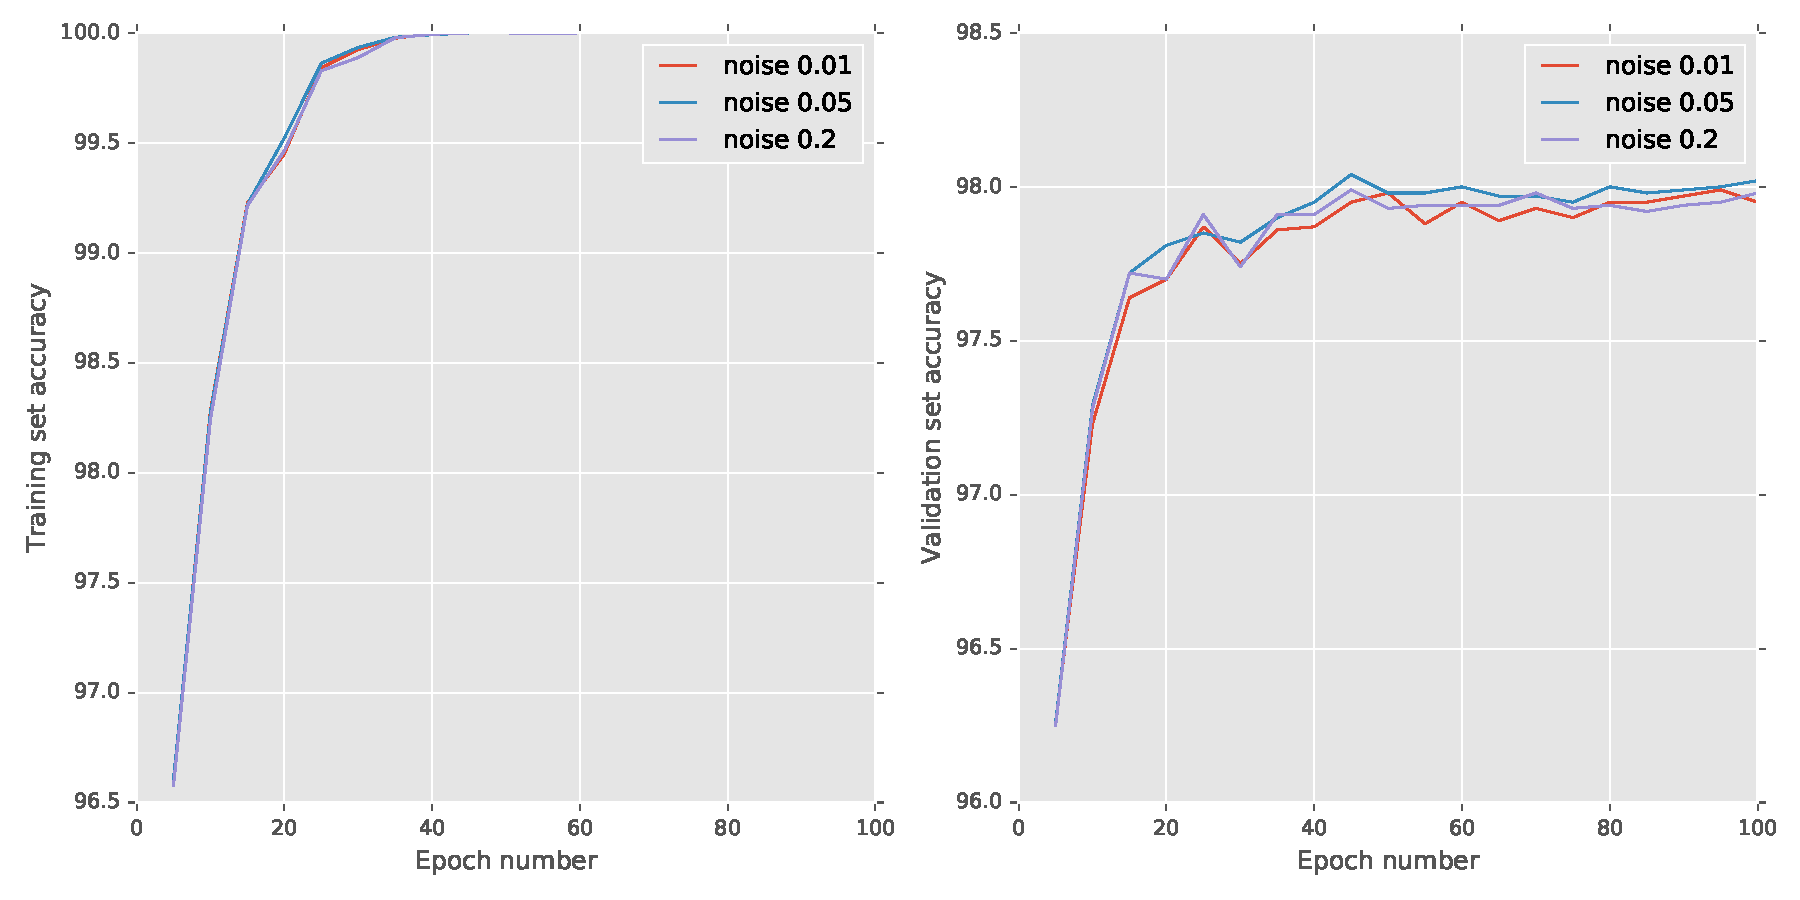
\includegraphics[width=\textwidth]{noise_compare_both.pdf}

  \caption{Effect of applying color variation to training data.}
  \label{fig:noise}
\end{figure}

Next technique that was expected to work quite well is zooming in/out the digits by a small extent. This should mimic people' writing styles and should allow the model to learn the shapes of the digits better. Different ranges of random zooms were explored in figure \ref{fig:zoom} and the results show an improvement compared to the baseline model.


\begin{figure}[H]
\centering
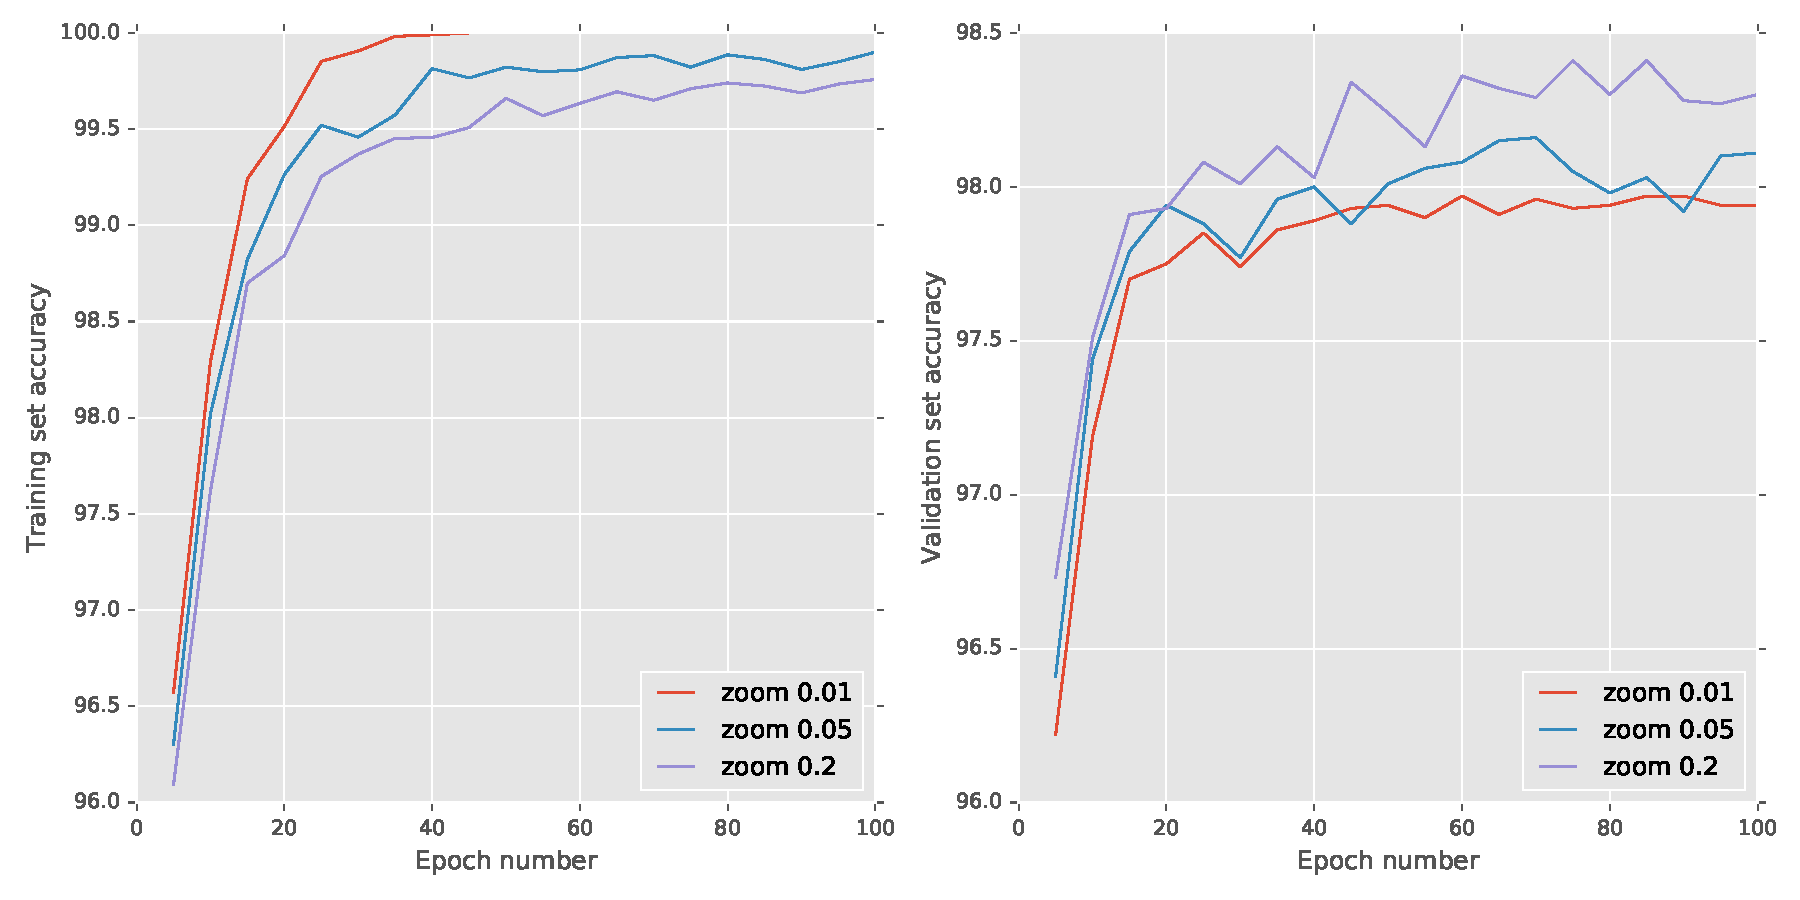
\includegraphics[width=\textwidth]{zoom_compare.pdf}

  \caption{Effect of applying zooming in/out to training data.}
  \label{fig:zoom}
\end{figure}

The last experiment for data augmentation explored whether combination of the well performing techniques above would perform better than each individually. For each data point to be augmented a random choice was made to either perform shift or zoom, as these improved performance individually. The best parameters for each augmentation technique were plotted against the baseline model as well as the combination of shift and zoom and the results are displayed on figure \ref{fig:comb}.

\begin{figure}[H]
\centering
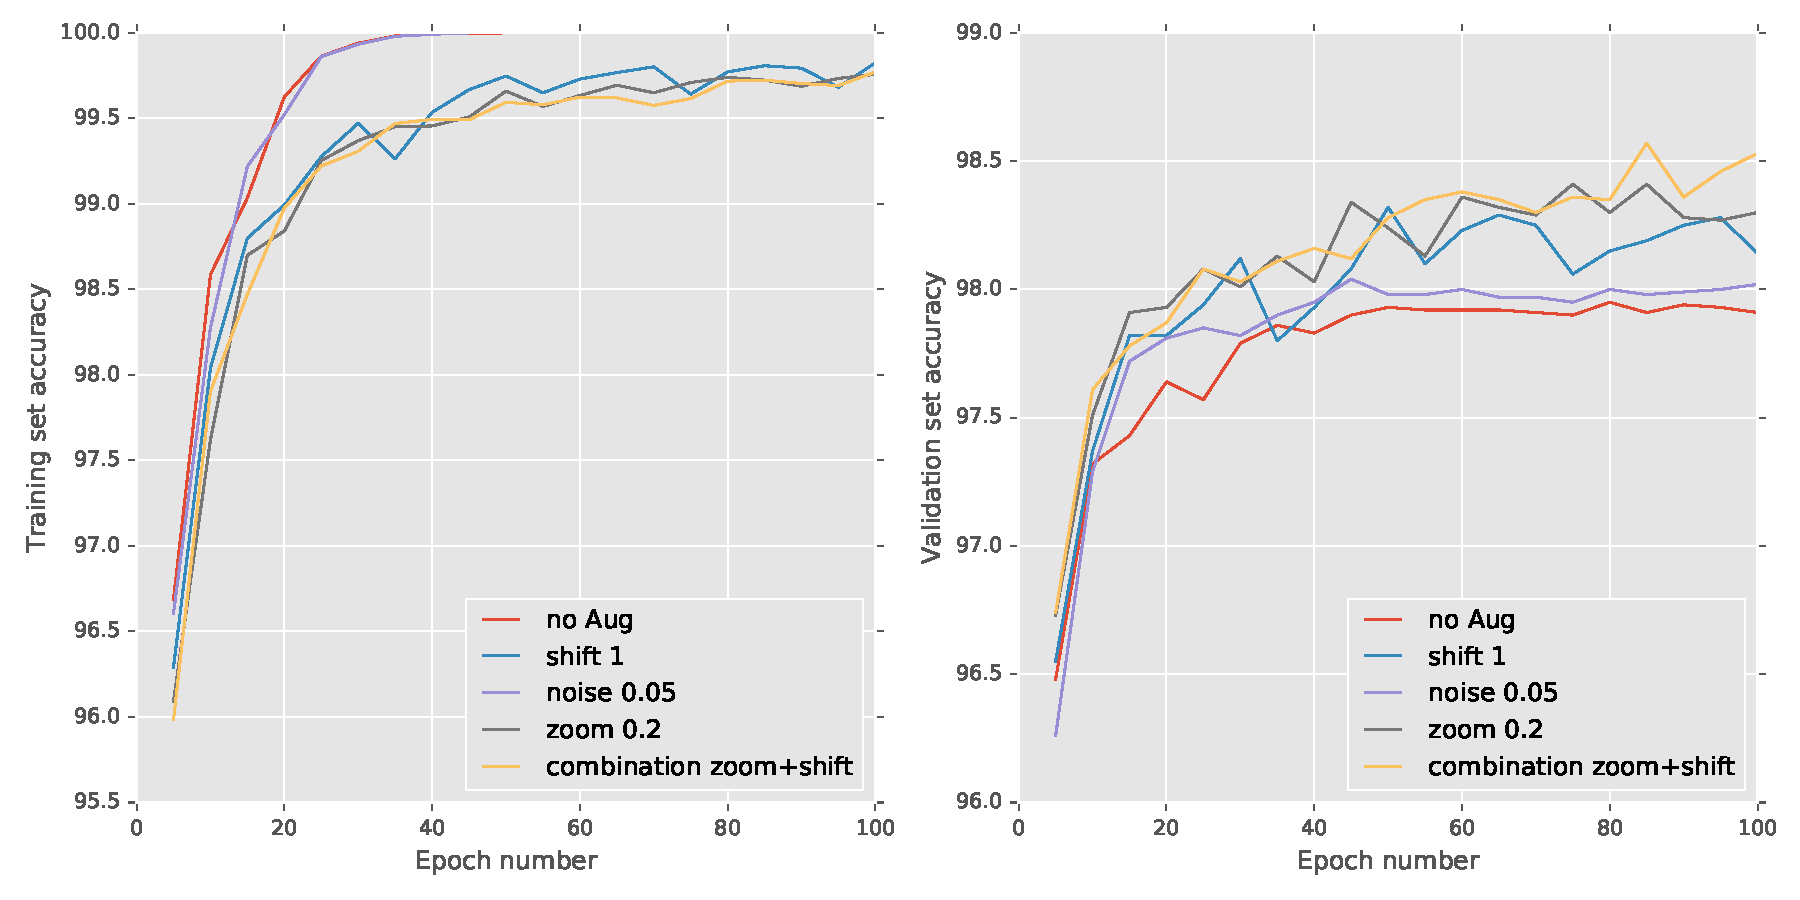
\includegraphics[width=\textwidth]{comb_compare.pdf}

  \caption{Comparison of augmentation techniques.}
  \label{fig:comb}
\end{figure}

The comparison of augmentation techniques clearly shows that data augmentation can result in a better final accuracy. Of the explored techniques color variations show minor improvement, whilst zoom and shift proved to be very effective. More importantly a combination of different augmentations has an even better effect than each method individually, resulting in more than 0.5\% improvement in accuracy.

\section*{Batch Normalization}

The effects of Batch normalization are explored in this section. Batch normalization is a technique which provides any input to a layer with inputs having zero mean/unit variance. It has been shown that if the inputs have been whitened (zero mean/unit variance) the networks tend to converge faster.

\[ x'^k = (x^k-E[x^k])/\sqrt{Var[x^k]+\epsilon}\] 

The equations show inputs to a layer can be normalised, x are the inputs, E is a mean and epsilon is a small constant, in this example set to 0.00001.

\[ y^k = \gamma^kx'+\beta^k\] 

Parameters gamma and beta serve to scale and shift the normalized values and can be learned in the process with an interesting case where the network is capable of 'unlearning' the batch normalization.

Different batch sizes and learning rates were explored. First with a small learning rate as in the experiments before, displayed on figure \ref{fig:batch}. 

A couple of observations can be made, first that very small and very large batch sizes do not perform well. This can be caused by the fact that when the batch size is too small, it does not represent all the classes properly. When the batch size is too large, the data points get normalized across resulting in mostly grey image. Batch size of 50 and 100 performed on par with base line, but was rather zig-zaggy. This is caused by the calculation of mean and variance during validation where both are calculated from the current batch. A more optimal solution would be to keep a global average mean and variance learned during training by for example moving average.



\begin{figure}[H]
\centering
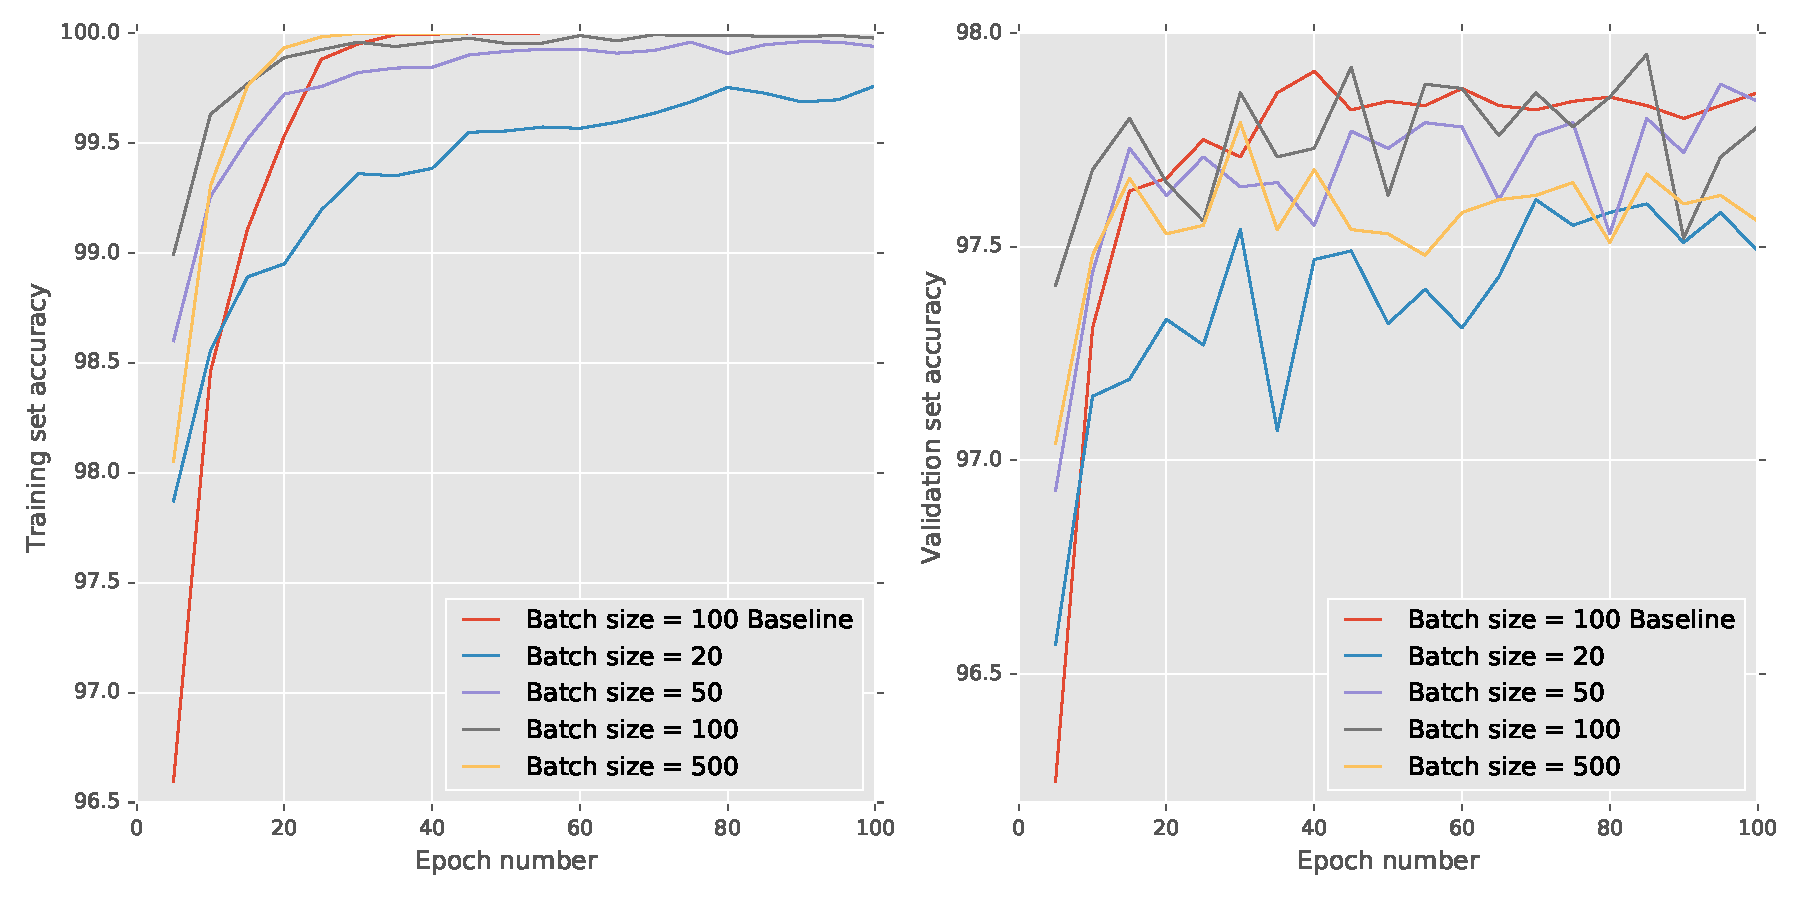
\includegraphics[width=\textwidth]{batch_compare.pdf}

  \caption{Batch normalization with learning rate 0.01 and no moving average}
  \label{fig:batch}
\end{figure}



Introducing an average mean and variance learned by an exponential moving average function during training indeed increases performance and smooths out the learning. The exponential moving average was chosen to give the last added values to contribute more than the first ones, as they should be more representative. The coefficient of how they contribute was arbitrarily was tested at 20\% and 5\%. The batch size comparisons with a moving average function for mean and variance is displayed on figures \ref{fig:batch2} and \ref{fig:batch3}. Showing that contribution of 5\% performs better, but this value could be further explored. With this parameter the batch normalization shows an improvement to the baseline model

\begin{figure}[H]
\centering
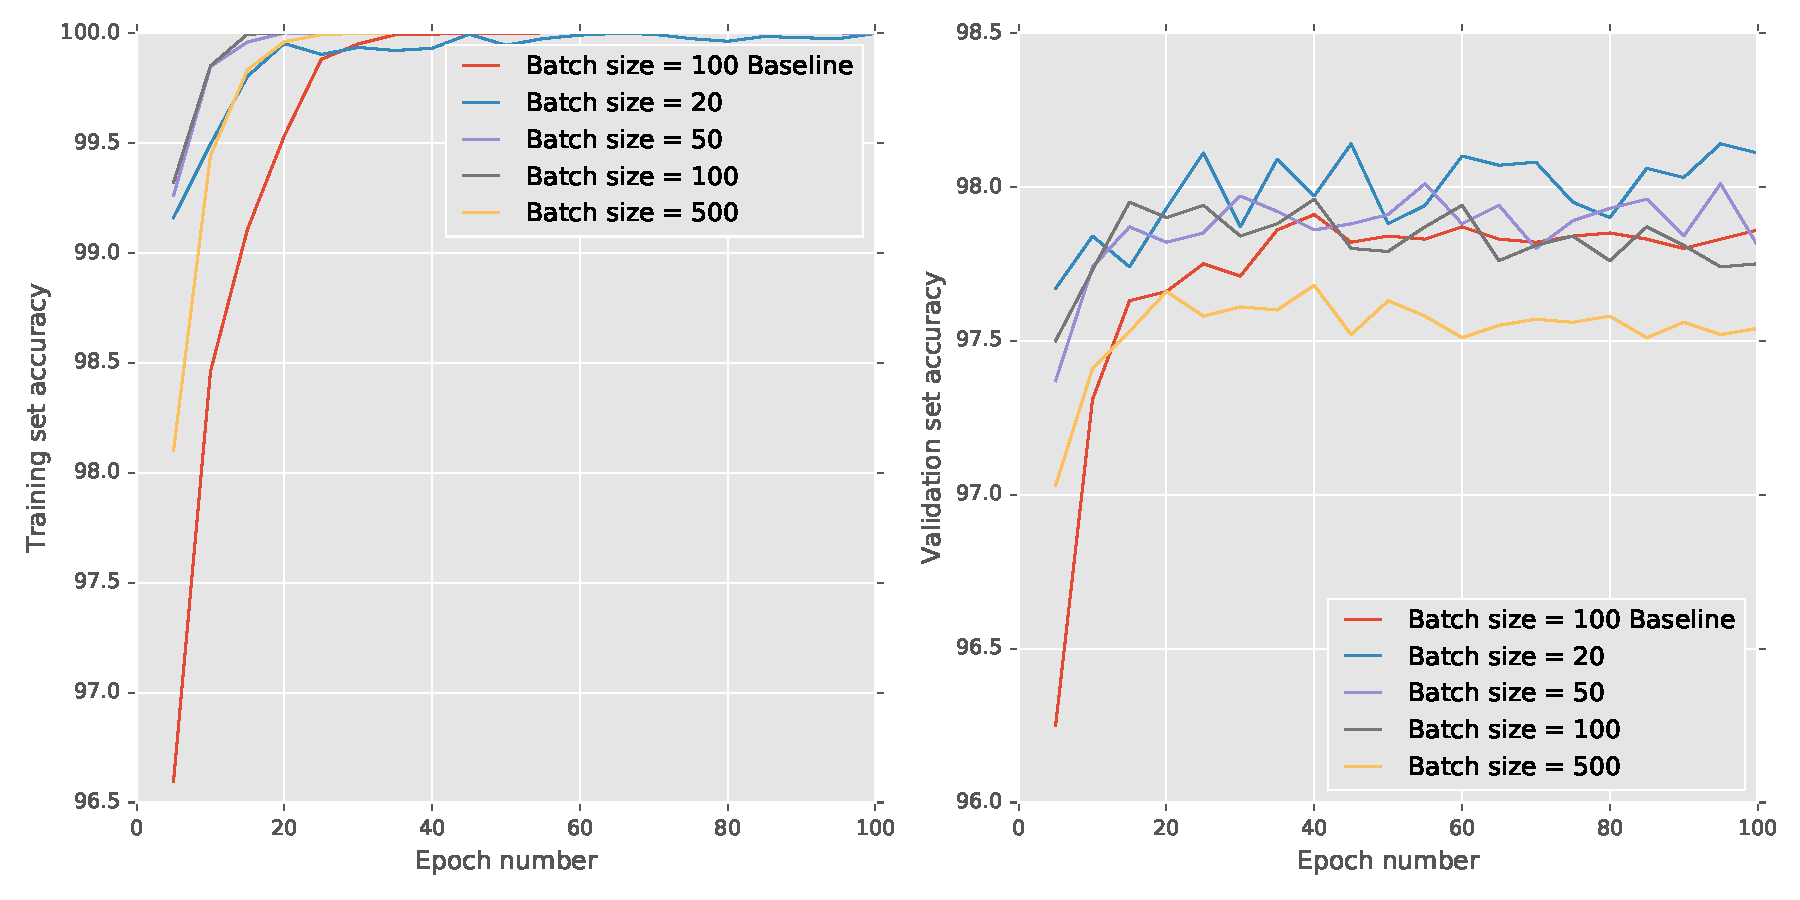
\includegraphics[width=\textwidth]{batch_compare_02.pdf}

  \caption{Batch normalization with learning rate 0.01 and moving average where new values contribute by 20\%}
  \label{fig:batch2}
\end{figure}


\begin{figure}[H]
\centering
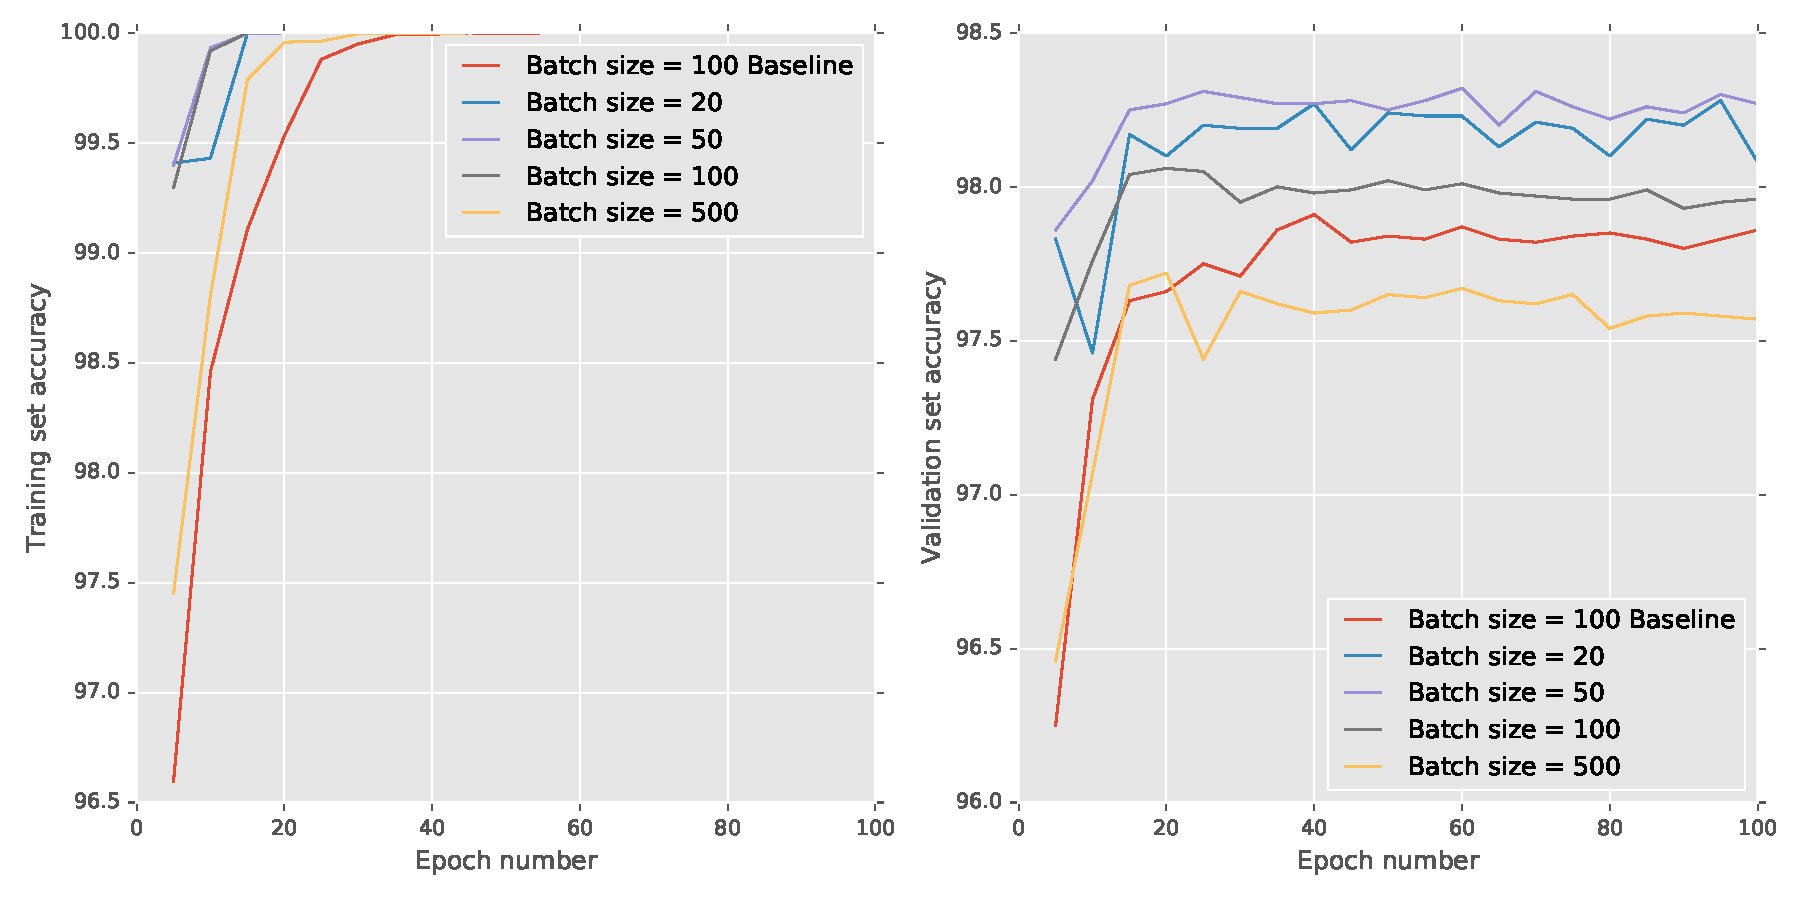
\includegraphics[width=\textwidth]{batch_compare05.pdf}

  \caption{Batch normalization with learning rate 0.01 and moving average where new values contribute by 5\%}
  \label{fig:batch3}
\end{figure}


An potential advantage of batch normalization was explored looking whether it allows for faster learning. The run with an increased learning rate to 0.1 and different batch sizes is displayed on figure \ref{fig:batchr}. The results show that batch normalization indeed allows for higher learning rates, clearly outperforming the baseline model.

\begin{figure}[H]
\centering
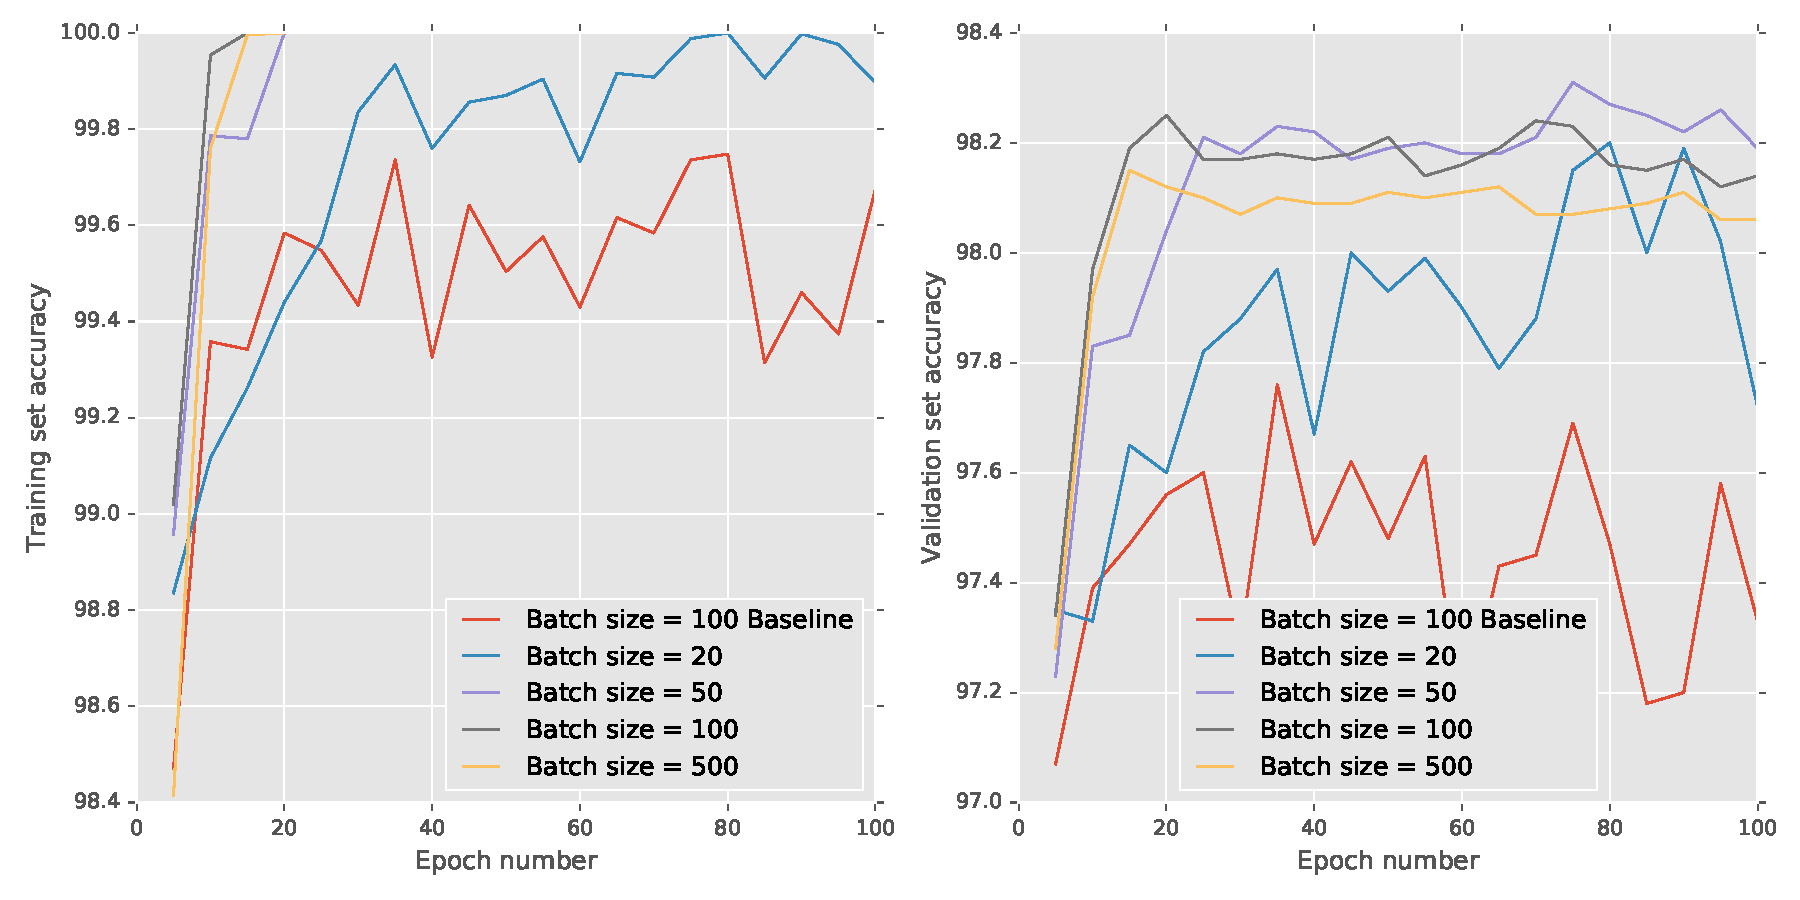
\includegraphics[width=\textwidth]{batch_compare_rate.pdf}

  \caption{Batch normalization with learning rate 0.01 and moving average where new values contribute by 5\%}
  \label{fig:batchr}
\end{figure}


\subsection*{Discussion and conclusion}
Three key topics were explored in this paper : activation layer choice, data augmentation and batch normalization. All three have proven their capability of increasing classification accuracy. Activation layer choice suggested using non-saturating Relu layers instead of sigmoid functions. Even basic data augmentation techniques showed to have a significant impact thanks to creating new, relevant data points based on the dataset. More importantly a combination of these should be used rather than just one individually as was showed during experiments. Batch normalization has been also shown to improve model classification accuracy as well as allowing for an increased learning rate.


\end{document}